\section{卷积光滑化}
\label{sec:weakd-convolution-smoothing}

阶跃函数$\mathbf 1_{(0,\infty)}$在原点断开。若把每一点的函数值换成它在一个小邻域内的加权平均，并让权重光滑地变化，得到的函数就不再有断点；邻域越小，平均值越接近原来的值。要把这个想法写成定理，先得规定哪些函数可以做局部平均、用什么函数做权重。

本章的点$x,y,z$都在欧氏空间$\mathbb R^d$中，作为积分变量使用，不加粗；$\lvert x\rvert$表示欧氏长度，$\mathrm dx$表示$d$维Lebesgue测度。$\Omega$总表示$\mathbb R^d$中的非空开集，$\operatorname{dist}(x,\Omega^{c})$表示$x$到补集$\Omega^{c}=\mathbb R^d\setminus\Omega$的距离；$\Omega=\mathbb R^d$时约定这个距离为$+\infty$。

\subsection{局部可积函数与测试函数}
\label{sec:weakd-local-integrability}

在一点附近做平均，只需要函数在这个邻域上可积，不需要它在整个区域上可积。考虑$(0,1)$上的$1/x$：它在靠近$0$处无界，整体积分发散；但在离$0$有一段距离的地方，它是有界连续函数，完全可以平均。下面的定义只要求这种局部控制。

\begin{definition}[局部可积]
\label{def:weakd-locally-integrable}
设$f$是$\Omega$上的可测函数，取实值或复值。若对每个紧集$K\subset\Omega$都有$\int_K\lvert f\rvert\,\mathrm dx<\infty$，就称$f$在$\Omega$上\term{局部可积}（locally integrable），记作$f\in L^1_{\mathrm{loc}}(\Omega)$。几乎处处相等的两个函数视为同一元素。
\end{definition}

定义只检查紧含于$\Omega$的集合，所以函数在边界附近可以任意增大。仍以$1/x$为例。$(0,1)$的紧子集$K$都落在某个$[a,b]$中，其中$0<a<b<1$，而$1/x$在其上不超过$1/a$，于是
\[
\int_K\frac{\mathrm dx}{x}\leq\frac{b-a}{a}<\infty .
\]
所以$1/x\in L^1_{\mathrm{loc}}(0,1)$。另一方面，
\[
\int_0^1\frac{\mathrm dx}{x}=+\infty ,
\]
它在$(0,1)$上不可积。

把同一个函数放到整条实轴上，紧区间$[-1,1]$上的积分就发散了，它不再局部可积。可见局部可积依赖于区域：边界在哪里，哪里就不受控制。

\paragraph{支撑与测试函数}
平均要用权重函数。为了让权重只读取区域内部的值，并且在后面的分部积分中不留下边界项，我们要求权重在边界附近恒为零。先把“恒为零的地方”说清楚。

\begin{definition}[支撑与测试函数]
\label{def:weakd-test-function}
函数$\varphi:\Omega\to\mathbb C$的\term{支撑}（support of a function）是集合$\{x\in\Omega:\varphi(x)\neq0\}$在$\mathbb R^d$中的闭包，记作$\operatorname{supp}\varphi$。$\Omega$上无穷次可微、支撑是紧集且含于$\Omega$的函数全体记作$C_c^\infty(\Omega)$，其中的函数称为\term{测试函数}（test function）。
\end{definition}

支撑是紧集并含于$\Omega$，意味着它与补集$\Omega^{c}$有正距离，因为紧集到不相交闭集的距离为正。于是存在$\delta>0$，使离边界不到$\delta$的点上测试函数恒为零。

测试函数$\varphi$在其支撑$K$上连续，因而有界。所以对$f\in L^1_{\mathrm{loc}}(\Omega)$，有
\begin{equation}
\Bigl\lvert\int_\Omega f\varphi\,\mathrm dx\Bigr\rvert\leq\Bigl(\sup_{K}\lvert\varphi\rvert\Bigr)\int_K\lvert f\rvert\,\mathrm dx<\infty .
\label{eq:weakd-local-pairing}
\end{equation}
这说明局部可积正是让“与测试函数相乘后积分”有意义的条件。改变$f$在零测集上的值不影响左端，所以这个积分读取的是几乎处处等价类的信息。

\paragraph{光滑隆起函数}
测试函数是否存在，需要构造才能回答。多项式、指数和三角函数都做不到：它们在一点的全部导数决定了整条实轴上的值，一旦在某个区间上恒为零，就处处为零。我们要找一个在某点所有导数都为零、却不恒为零的光滑函数。

令
\[
E(s)=\exp(-1/s)\quad(s>0),\qquad E(s)=0\quad(s\leq0).
\]
先看它在$s>0$处的各阶导数。对$k$归纳可以写出
\[
E^{(k)}(s)=P_k(1/s)\,\exp(-1/s),\qquad s>0,
\]
其中$P_k$是多项式。$k=0$时$P_0=1$。由$k$到$k+1$时求一次导，得到
\[
\frac{\mathrm d}{\mathrm ds}\Bigl[P_k(1/s)\,\mathrm e^{-1/s}\Bigr]
=\frac{1}{s^2}\Bigl[P_k(1/s)-P_k'(1/s)\Bigr]\mathrm e^{-1/s},
\]
方括号外的因子$s^{-2}$与方括号内的式子合起来仍是$1/s$的多项式。

再看$s\to0^+$时的行为。令$t=1/s\to+\infty$，对每个整数$m\geq0$有
\[
s^{-m}\,\mathrm e^{-1/s}=t^m\mathrm e^{-t}\to0 ,
\]
指数压过任意多项式，所以$E^{(k)}(s)\to0$（$s\to0^+$）。

最后在$s=0$处逐阶检查导数定义。设已知$E^{(k)}(0)=0$。左侧的差商为零，右侧的差商是
\[
\frac{E^{(k)}(s)-0}{s}=\frac1s\,P_k(1/s)\,\mathrm e^{-1/s}\to0 .
\]
所以$E^{(k+1)}(0)=0$。这样$E$在实轴上无穷次可微，并且在原点的全部导数为零，它的Taylor级数在原点恒为零，却不等于$E$本身。

把$s$换成$1-\lvert x\rvert^2$，得到
\begin{equation}
\psi(x)=E\bigl(1-\lvert x\rvert^2\bigr)=
\begin{cases}
\exp\Bigl(-\dfrac{1}{1-\lvert x\rvert^2}\Bigr),&\lvert x\rvert<1,\\
0,&\lvert x\rvert\geq1 .
\end{cases}
\label{eq:weakd-bump}
\end{equation}
$\lvert x\rvert^2=x_1^2+\cdots+x_d^2$是多项式，与光滑函数$E$复合后仍光滑。$\psi$在开单位球内为正，在球外为零，支撑是闭单位球。这样的函数称为\term{隆起函数}（bump function）。

隆起函数可以放到任意内点附近。设$x_0\in\Omega$，取$0<r<\operatorname{dist}(x_0,\Omega^{c})$，令
\[
\varphi(x)=\psi\Bigl(\frac{x-x_0}{r}\Bigr).
\]
它在开球$B(x_0,r)$内为正，支撑是闭球$\overline B(x_0,r)$，紧且含于$\Omega$，所以$\varphi\in C_c^\infty(\Omega)$。因此每个内点附近都有测试函数，而且可以把支撑压缩到任意小的球内。

图~\ref{fig:weakd-bump}按这三步画出构造。左图中$E$在原点左侧为零，右侧从零开始上升，接合处没有任何折痕；中图把两个这样的接合点放在$\pm1$，得到一个鼓包；右图把鼓包平移、缩小，放进区域$\Omega$内部。

\begin{BookInlineFigure}
  \centering
  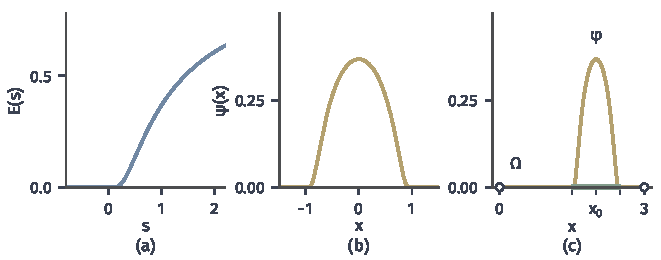
\includegraphics[width=112mm]{figures/04-spaces-measures-and-geometry/02-measure/matplotlib/weakd-bump/figure.pdf}
  \caption{隆起函数的构造，一维情形。(a)~$E(s)$在$s\leq0$处为零，在$s>0$处为$\exp(-1/s)$。(b)~隆起函数$\psi$的支撑是$[-1,1]$，峰值$\mathrm e^{-1}\approx0.368$。(c)~区域$\Omega=(0,3)$内的测试函数$\varphi(x)=\psi((x-x_0)/r)$，这里$x_0=2$，$r=0.5$；横轴上的绿色线段是支撑$[1.5,2.5]$，两个空心圆表示$\Omega$的端点不属于$\Omega$。}
  \label{fig:weakd-bump}
\end{BookInlineFigure}

\subsection{卷积}
\label{sec:weakd-convolution}

局部平均要把$f$在$x$附近的值按某个权重加起来，权重只依赖于被读取的点相对$x$的位置。这件事在数列上是熟悉的滑动平均，我们先从数列看起。

把一个双向无穷的数列看成向量$a=[\ldots,a_{-1},a_0,a_1,a_2,\ldots]$，再取一组权重$w_{-1}=w_1=\tfrac14$，$w_0=\tfrac12$，其余$w_j=0$。滑动平均把第$k$个分量换成它和两个邻居的加权平均：
\begin{equation}
b_k=\sum_{j}w_j\,a_{k-j}=\tfrac14a_{k+1}+\tfrac12a_k+\tfrac14a_{k-1}.
\label{eq:weakd-moving-average}
\end{equation}
下面用一个台阶状的向量手算一遍，它在$k\leq0$处为$0$，在$k\geq1$处为$1$。把四个相邻的下标代入式~\eqref{eq:weakd-moving-average}，得到
\[
b_{-1}=0,\quad b_0=\tfrac14,\quad b_1=\tfrac34,\quad b_2=1.
\]

台阶从一步跳变摊成了两级小台阶，如图~\ref{fig:weakd-moving-average}。权重的总和是$1$，所以常数向量经过平均不变；这里在$k\leq-1$处$b_k=0$，在$k\geq2$处$b_k=1$，正是因为这些位置的三个邻居都相同。

\begin{BookInlineFigure}
  \centering
  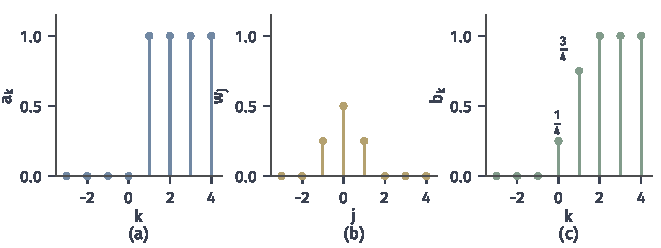
\includegraphics[width=112mm]{figures/04-spaces-measures-and-geometry/02-measure/matplotlib/weakd-moving-average/figure.pdf}
  \caption{数列上的滑动平均。(a)~台阶状的向量$a$。(b)~权重$w_{-1}=w_1=\frac14$，$w_0=\frac12$，总和为$1$。(c)~平均后的向量$b$：跳变被摊开到两个位置，离跳变较远的分量不变。}
  \label{fig:weakd-moving-average}
\end{BookInlineFigure}

现在让下标连续变化，把函数看成“每个点占一个分量”的向量。分量$a_k$变成函数值$f(x)$，权重$w_j$变成权重函数$g(z)$，求和变成积分。表~\ref{tab:weakd-dictionary}列出对应关系，其中式~\eqref{eq:weakd-moving-average}对应的连续形式就是卷积。

\begin{BookInlineTable}
  \centering
  \begin{tabular}{@{}ll@{}}
    \toprule
    数列 & 函数\\
    \midrule
    下标$k\in\mathbb Z$ & 点$x\in\mathbb R^d$\\
    分量$a_k$ & 函数值$f(x)$\\
    权重$w_j$，$\sum_jw_j=1$ & 权重函数$g(z)$，$\int g\,\mathrm dz=1$\\
    平移$k\mapsto k-j$ & 平移$x\mapsto x-z$\\
    $b_k=\sum_jw_j\,a_{k-j}$ & $(f*g)(x)=\int g(z)\,f(x-z)\,\mathrm dz$\\
    \bottomrule
  \end{tabular}
  \caption{滑动平均与卷积的对应。}
  \label{tab:weakd-dictionary}
\end{BookInlineTable}

类比有一处要改。数列的每个分量都有自己的权重，改动一个分量，平均值就可能变；函数的单个点在积分中没有权重，改动一个点不影响平均。所以卷积只读取函数的几乎处处等价类，这正是我们想要的。

\paragraph{平移与缩放的积分规则}
卷积的计算反复用到变量替换，先核对Lebesgue积分在平移、反射和缩放下怎样变化。设$h\in\mathbb R^d$，$a\neq0$，记$\lambda_d$为$d$维Lebesgue测度。

第~\ref{chap:measure}章的Lebesgue外测度是用可数个矩形覆盖的总体积取下确界得到的。矩形$R=\prod_{i}[\alpha_i,\beta_i]$平移$h$后仍是矩形，体积不变；关于原点反射后也是矩形，体积不变；乘以$a$后各边长乘$\lvert a\rvert$，体积乘$\lvert a\rvert^d$。集合$A$的覆盖与$A+h$、$-A$、$aA$的覆盖一一对应，总体积按同样的比例变化。

可测性判据中的检验集合也随之一一对应，因此可测集映成可测集，并且
\[
\lambda_d(A+h)=\lambda_d(A),\quad\lambda_d(-A)=\lambda_d(A),\quad\lambda_d(aA)=\lvert a\rvert^d\lambda_d(A).
\]

把集合的规则推广到函数。对指示函数$f=\mathbf 1_A$，有
\[
f(x-h)=\mathbf 1_{A+h}(x),\quad f(-x)=\mathbf 1_{-A}(x),\quad f(x/a)=\mathbf 1_{aA}(x),
\]
于是集合的规则就是函数的等式。由线性性推广到非负简单函数，再取递增的简单函数逼近并用单调收敛定理，得到对非负可测$f$成立的
\begin{equation}
\begin{gathered}
\int f(x-h)\,\mathrm dx=\int f(x)\,\mathrm dx,\qquad
\int f(-x)\,\mathrm dx=\int f(x)\,\mathrm dx,\\
\int f\Bigl(\frac xa\Bigr)\mathrm dx=\lvert a\rvert^d\int f(x)\,\mathrm dx .
\end{gathered}
\label{eq:weakd-translation-scaling}
\end{equation}
可积函数分正负部、实部与虚部处理，等式仍成立。缩放规则中的因子$\lvert a\rvert^d$将用来保持磨光核的总积分为$1$。

\paragraph{卷积的定义}
在$\mathbb R^d$上取两个可积函数$f,g$。我们希望对每个$x$计算
\begin{equation}
(f*g)(x)=\int_{\mathbb R^d}f(x-y)\,g(y)\,\mathrm dy .
\label{eq:weakd-convolution}
\end{equation}
右端有定义时，称$f*g$为$f$与$g$的\term{卷积}（convolution）。它把$g$当作权重，对$f$在$x-y$处的值累计。被积函数是两个可积函数之积，不一定可积，所以先要说明对哪些$x$右端有意义。

可测性要先处理。可测函数在一个Borel零测集外与某个Borel函数相等（第~\ref{chap:measure}章的完备化），先设$f,g$是Borel函数，则$(x,y)\mapsto f(x-y)g(y)$是$\mathbb R^{2d}$上的Borel函数，因为映射$(x,y)\mapsto x-y$连续。

若$f$在Borel零测集$N$之外被改值，被改动的点落在$\{(x,y):x-y\in N\}$中。这个集合对每个固定的$y$的截面是$N+y$，测度为零，由Tonelli定理它是$\mathbb R^{2d}$中的零测集。$g$的改值同样只涉及零测集$\mathbb R^d\times N'$，所以都不影响下面的积分。

\begin{theorem}[可积函数的卷积]
\label{thm:weakd-convolution-l1}
设$f,g$在$\mathbb R^d$上可积。则对几乎每个$x\in\mathbb R^d$，函数$y\mapsto f(x-y)g(y)$可积，由式~\eqref{eq:weakd-convolution}定义的$f*g$几乎处处有定义、可积，并且
\begin{equation}
\int_{\mathbb R^d}\lvert(f*g)(x)\rvert\,\mathrm dx\leq\Bigl(\int_{\mathbb R^d}\lvert f\rvert\,\mathrm dx\Bigr)\Bigl(\int_{\mathbb R^d}\lvert g\rvert\,\mathrm dx\Bigr).
\label{eq:weakd-young-l1}
\end{equation}
此外$f*g=g*f$几乎处处成立。
\end{theorem}

\begin{proof}
对非负函数$(x,y)\mapsto\lvert f(x-y)\rvert\lvert g(y)\rvert$用Tonelli定理，先对$x$积分。由式~\eqref{eq:weakd-translation-scaling}的平移规则，内层对$x$的积分等于$\int\lvert f\rvert$，与$y$无关，所以
\[
\begin{aligned}
\int\!\!\int\lvert f(x-y)\rvert\,\lvert g(y)\rvert\,\mathrm dy\,\mathrm dx
&=\int\lvert g(y)\rvert\Bigl(\int\lvert f(x-y)\rvert\,\mathrm dx\Bigr)\mathrm dy\\
&=\int\lvert f\rvert\,\mathrm dx\cdot\int\lvert g\rvert\,\mathrm dy<\infty .
\end{aligned}
\]

左端按另一种次序是$\int G(x)\,\mathrm dx$，其中
\[
G(x)=\int\lvert f(x-y)\,g(y)\rvert\,\mathrm dy .
\]
非负函数积分有限，所以$G(x)<\infty$对几乎每个$x$成立，这些$x$处$y\mapsto f(x-y)g(y)$可积。

被积函数在$\mathbb R^{2d}$上绝对可积，由Fubini定理，$x\mapsto(f*g)(x)$在例外零测集外有定义且可测（例外集上取零），并且$\lvert(f*g)(x)\rvert\leq G(x)$。对$x$积分即得式~\eqref{eq:weakd-young-l1}。

交换律来自对固定的$x$作替换$y\mapsto x-y$。它是反射与平移的复合，由式~\eqref{eq:weakd-translation-scaling}不改变积分，于是
\[
\int f(x-y)\,g(y)\,\mathrm dy=\int f(y)\,g(x-y)\,\mathrm dy .
\]
\end{proof}

两个可积性条件都不能少。若只假设$f,g$局部可积，卷积可以处处发散：$\mathbb R$上$f=g=1$时，对每个$x$都有
\[
\int_{\mathbb R}f(x-y)\,g(y)\,\mathrm dy=\int_{\mathbb R}1\,\mathrm dy=+\infty .
\]
式~\eqref{eq:weakd-young-l1}的证明正是靠两个绝对积分的乘积有限，Tonelli定理才给出几乎处处有限的内层积分。下一小节的磨光核紧支撑且有界，那时只需要$f$局部可积，因为每个$x$处的积分只读取$f$在一个紧集上的值。

下面的例子可以逐点算出，它把权重的滑动过程完整走一遍。

\begin{example}[两个盒函数的卷积]
\label{ex:weakd-box-convolution}
取$d=1$，$f=g=\mathbf 1_{[0,1]}$。由交换律，用形式$\int f(y)g(x-y)\,\mathrm dy$来算。固定$x$，$g(x-y)=1$当且仅当$x-y\in[0,1]$，也就是$y\in[x-1,x]$。所以卷积值就是两段的重叠长度：
\[
(f*g)(x)=\lambda_1\bigl([0,1]\cap[x-1,x]\bigr).
\]
当$0\leq x\leq1$时重叠区间是$[0,x]$，当$1\leq x\leq2$时重叠区间是$[x-1,1]$，其余情形没有重叠。于是
\[
(f*g)(x)=\begin{cases}x,&0\leq x\leq1,\\2-x,&1\leq x\leq2,\\0,&\text{其余情形}.\end{cases}
\]
三角形的面积是$\frac12\cdot2\cdot1=1$，恰好等于$\int f\cdot\int g=1$，式~\eqref{eq:weakd-young-l1}在这里取等号。
\end{example}

图~\ref{fig:weakd-convolution-box}中，蓝色盒子固定，黄色盒子随$x$向右滑动，绿色部分的长度就是卷积值。两个不连续的函数卷积后成为连续函数，这是卷积光滑作用的最简单表现：滑动权重的边缘越过跳点时，重叠长度是连续变化的。

\begin{BookInlineFigure}
  \centering
  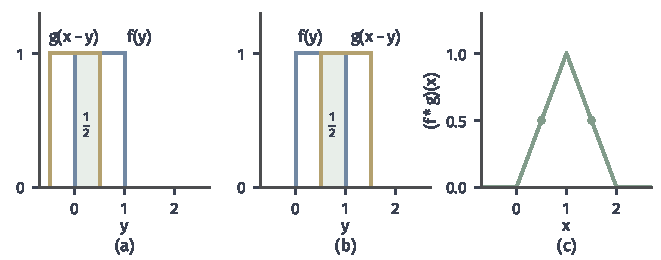
\includegraphics[width=112mm]{figures/04-spaces-measures-and-geometry/02-measure/matplotlib/weakd-convolution-box/figure.pdf}
  \caption{盒函数的卷积。(a)~$x=0.5$时固定盒子$f(y)$与滑动盒子$g(x-y)$重叠的绿色部分长$\frac12$。(b)~$x=1.5$时重叠长度同样是$\frac12$。(c)~卷积结果是$[0,2]$上的三角形，两个圆点是(a)、(b)的读数。}
  \label{fig:weakd-convolution-box}
\end{BookInlineFigure}

\subsection{局部磨光}
\label{sec:weakd-local-mollification}

现在把隆起函数归一化为权重，对局部可积函数做局部平均。由于$f$只在$\Omega$上有定义，平均的邻域必须留在$\Omega$内，这决定了磨光函数的定义域。

\paragraph{磨光核与磨光}
令$c_d=\int_{\mathbb R^d}\psi\,\mathrm dx>0$，其中$\psi$是式~\eqref{eq:weakd-bump}的隆起函数，并令
\begin{equation}
\rho(x)=c_d^{-1}\psi(x),\qquad\rho_\varepsilon(x)=\varepsilon^{-d}\rho\Bigl(\frac x\varepsilon\Bigr)\quad(\varepsilon>0).
\label{eq:weakd-mollifier}
\end{equation}
$\rho_\varepsilon$光滑、非负，支撑是闭球$\overline B(0,\varepsilon)$。由式~\eqref{eq:weakd-translation-scaling}的缩放规则，
\[
\int\rho_\varepsilon\,\mathrm dx=\varepsilon^{-d}\cdot\varepsilon^d\int\rho\,\mathrm dx=1 .
\]

$\varepsilon$减小时支撑收缩，高度按$\varepsilon^{-d}$增大，总积分保持为$1$。下面的论证只用到$\rho$光滑、非负、积分为$1$并支撑于闭单位球，任何满足这些条件的核都可以代替它；我们把这类函数称为\term{磨光核}（mollifier）。

一维时$c_1\approx0.4440$，峰值$\rho_\varepsilon(0)\approx0.829/\varepsilon$。后面的手算还要用到$\rho$的两个矩：
\[
m_1=\int_{-1}^{1}\lvert u\rvert\rho(u)\,\mathrm du\approx0.3345,\qquad
m_2=\int_{-1}^{1}u^2\rho(u)\,\mathrm du\approx0.1581 .
\]
这些数值由数值积分得到。$\rho$是偶函数，所以$\int u\rho(u)\,\mathrm du=0$。

平均的邻域要留在$\Omega$内，因此只能在离边界足够远的点上做平均。记
\[
\Omega_\varepsilon=\{x\in\Omega:\operatorname{dist}(x,\Omega^{c})>\varepsilon\},
\]
它是开集。对$f\in L^1_{\mathrm{loc}}(\Omega)$与$x\in\Omega_\varepsilon$，闭球$\overline B(x,\varepsilon)$是$\Omega$内的紧集，定义
\begin{equation}
\begin{aligned}
f_\varepsilon(x)&=\int_\Omega\rho_\varepsilon(x-y)\,f(y)\,\mathrm dy\\
&=\int_{\lvert z\rvert\leq\varepsilon}\rho_\varepsilon(z)\,f(x-z)\,\mathrm dz ,\qquad x\in\Omega_\varepsilon ,
\end{aligned}
\label{eq:weakd-mollification}
\end{equation}
称为$f$的\term{磨光}（mollification）。

被积函数在紧集$\overline B(x,\varepsilon)$外为零，由式~\eqref{eq:weakd-local-pairing}积分有限；第二个等号是替换$z=x-y$。因为$\rho_\varepsilon\geq0$且$\int\rho_\varepsilon=1$，$f_\varepsilon(x)$是$f$在球$B(x,\varepsilon)$上的加权平均，权重集中在中心附近。$\Omega=\mathbb R^d$且$f$可积时，$f_\varepsilon=f*\rho_\varepsilon$就是上一小节的卷积。

图~\ref{fig:weakd-interior}(a)说明为什么定义域要缩小：点$x$的平均球完全落在$\Omega$内，可以计算；点$x'$的平均球越过了边界，要用到$f$没有定义的地方。

\begin{BookInlineFigure}
  \centering
  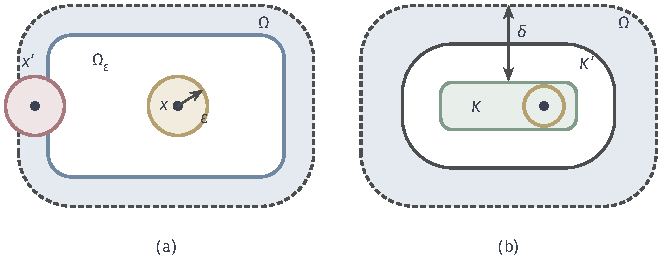
\includegraphics[width=112mm]{figures/04-spaces-measures-and-geometry/02-measure/tikz/weakd-interior/figure.pdf}
  \caption{磨光的定义域与局部逼近中的紧集。虚线是开集$\Omega$的边界。(a)~白色区域是$\Omega_\varepsilon$，灰蓝色环带上的点离边界不超过$\varepsilon$。黄色球$B(x,\varepsilon)$留在$\Omega$内，红色球越出$\Omega$，所以$x'\notin\Omega_\varepsilon$。(b)~紧集$K$（绿色）到$\Omega^{c}$的距离为$\delta$，$K'$是$K$的$\delta/2$邻域。半径小于$\delta/2$的黄色球以$K$中点为心时，都留在$K'$内。}
  \label{fig:weakd-interior}
\end{BookInlineFigure}

\paragraph{磨光函数的光滑性}
磨光把$x$只放在核里，被积的$f(y)$与$x$无关。所以对$x$求导时，可以把导数全部移到光滑的核上；需要检查的只是积分号下求导的条件。

\begin{theorem}[磨光函数光滑]
\label{thm:weakd-mollification-smooth}
设$f\in L^1_{\mathrm{loc}}(\Omega)$，$\varepsilon>0$。则$f_\varepsilon\in C^\infty(\Omega_\varepsilon)$，并且对每个多重指标$\alpha$，
\begin{equation}
\partial^\alpha f_\varepsilon(x)=\int_\Omega(\partial^\alpha\rho_\varepsilon)(x-y)\,f(y)\,\mathrm dy ,\qquad x\in\Omega_\varepsilon .
\label{eq:weakd-mollifier-derivative}
\end{equation}
这里\term{多重指标}（multi-index）$\alpha=(\alpha_1,\ldots,\alpha_d)$是非负整数组，$\lvert\alpha\rvert=\alpha_1+\cdots+\alpha_d$称为它的阶数，$\partial^\alpha$表示依次对第$j$个坐标求$\alpha_j$次偏导；$\alpha=0$时$\partial^\alpha$是恒等运算。
\end{theorem}

\begin{proof}
固定$x_0\in\Omega_\varepsilon$，取$r>0$使$\operatorname{dist}(x_0,\Omega^{c})>\varepsilon+2r$，再令$K=\overline B(x_0,\varepsilon+r)$，它是$\Omega$内的紧集。对$x\in B(x_0,r)$，若$\rho_\varepsilon(x-y)\neq0$，则$\lvert y-x\rvert<\varepsilon$，从而$y\in K$。因此在这个参数邻域内，被积函数可以写成$\rho_\varepsilon(x-y)f(y)\mathbf 1_K(y)$。

先求一个坐标方向的偏导数。对固定的$y$，$x\mapsto\rho_\varepsilon(x-y)f(y)$光滑，对$x_j$的偏导数是$(\partial_j\rho_\varepsilon)(x-y)f(y)$，其绝对值不超过
\[
M_j\,\lvert f(y)\rvert\,\mathbf 1_K(y),\qquad M_j=\sup_{\mathbb R^d}\lvert\partial_j\rho_\varepsilon\rvert<\infty .
\]
这个上界与$x\in B(x_0,r)$无关，并且由$f$局部可积而可积。沿第$j$个坐标的参数区间应用第~\ref{chap:integration}章的积分号下求导定理，得到式~\eqref{eq:weakd-mollifier-derivative}在$\lvert\alpha\rvert=1$时成立。

右端仍是同一形式的积分，只是核换成了光滑紧支撑函数$\partial_j\rho_\varepsilon$，支撑仍在$\overline B(0,\varepsilon)$内。对阶数归纳，重复上面的论证即得全部偏导数存在并满足式~\eqref{eq:weakd-mollifier-derivative}。

每个偏导数又是这种积分，被积函数关于$x$连续，并被同一个可积函数控制，由含参积分的连续性定理，它在$B(x_0,r)$上连续。$x_0$任意，所以$f_\varepsilon\in C^\infty(\Omega_\varepsilon)$。
\end{proof}

光滑性完全来自核，与$f$本身是否连续无关。下面在一维手算$f(x)=\lvert x\rvert$的磨光，$\Omega=\mathbb R$，看光滑化具体做了什么。

设$x\geq\varepsilon$。此时$\lvert z\rvert\leq\varepsilon$推出$x-z\geq0$，所以$\lvert x-z\rvert=x-z$。代入式~\eqref{eq:weakd-mollification}，并用$\int\rho_\varepsilon=1$、$\int z\rho_\varepsilon(z)\,\mathrm dz=0$，得到
\[
f_\varepsilon(x)=\int_{\lvert z\rvert\leq\varepsilon}\rho_\varepsilon(z)\,(x-z)\,\mathrm dz=x .
\]
$x\leq-\varepsilon$时同理得$f_\varepsilon(x)=-x$，所以在$\lvert x\rvert\geq\varepsilon$处磨光没有改变函数。

尖点处的值是$\rho_\varepsilon$的一阶矩。取$x=0$，再作替换$z=\varepsilon u$，得到
\[
f_\varepsilon(0)=\int_{\lvert z\rvert\leq\varepsilon}\rho_\varepsilon(z)\,\lvert z\rvert\,\mathrm dz=\varepsilon m_1 .
\]
$\varepsilon=0.5$时这个值约为$0.167$，图~\ref{fig:weakd-mollifier}(b)标出了它。同样的计算用于符号函数：在$\lvert x\rvert\geq\varepsilon$处，它的磨光等于自身；在原点，被积函数是奇函数，磨光值为$0$。

\begin{BookInlineFigure}
  \centering
  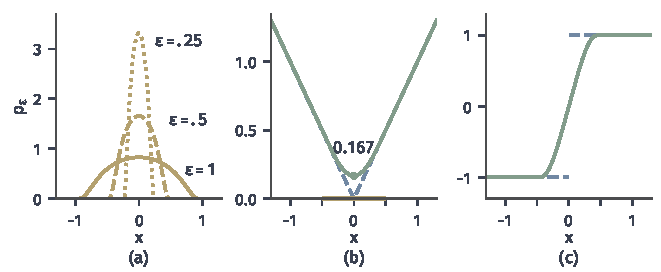
\includegraphics[width=112mm]{figures/04-spaces-measures-and-geometry/02-measure/matplotlib/weakd-mollifier/figure.pdf}
  \caption{一维磨光。(a)~磨光核$\rho_\varepsilon$，$\varepsilon=1,0.5,0.25$：支撑为$[-\varepsilon,\varepsilon]$，峰值约$0.829/\varepsilon$，面积均为$1$。(b)~$\lvert x\rvert$（蓝色虚线）与它的磨光（绿色实线），$\varepsilon=0.5$：尖点被抹平，原点值约$0.167$，横轴上黄色线段是改动发生的范围$[-\varepsilon,\varepsilon]$，其外两者重合。(c)~$\operatorname{sgn}x$与它的磨光，$\varepsilon=0.5$：后者光滑地从$-1$升到$1$，恰好是(b)中绿色曲线的导数。}
  \label{fig:weakd-mollifier}
\end{BookInlineFigure}

\subsection{平移的积分连续性}
\label{sec:weakd-translation-continuity}

磨光值$f_\varepsilon(x)$是$f(x-z)$在$\lvert z\rvert\leq\varepsilon$上的平均，所以$f_\varepsilon-f$由“把$f$平移一小段后与原来差多少”控制。逐点看，平移误差可以很大：阶跃函数平移后，跳点附近的值从$0$变成$1$。但改变的只是一段长度为$\lvert h\rvert$的区间，积分误差仍然小。

图~\ref{fig:weakd-translation}(a)画的是$\mathbf 1_{[0,1]}$平移$h=0.2$的情形。在两侧的红色条带上，逐点误差都等于$1$，一点也不小；但条带总宽只有$2h=0.4$，积分误差就是$0.4$，随$h$趋于零。下面要证明，对每个可积函数，平移引起的积分误差都随平移量趋于零。

\paragraph{集合的开集外逼近与紧集内逼近}
可积函数可以由简单函数逼近，简单函数由有限测度集合的指示函数组成。所以问题先归结为集合：一个有限测度可测集能否用一些矩形的有限并很好地近似。下面先从外测度的定义出发，用开集从外面、用紧集从里面夹住这个集合。

\begin{lemma}[Lebesgue测度的外逼近与内逼近]
\label{lem:weakd-regularity}
设$A\subset\mathbb R^d$可测且$\lambda_d(A)<\infty$，$\eta>0$。则存在开集$U\supset A$与紧集$K\subset A$，使$\lambda_d(U\setminus A)<\eta$且$\lambda_d(A\setminus K)<\eta$。
\end{lemma}

\begin{proof}
先做外逼近。按外测度的定义，存在可数个矩形$R_k$覆盖$A$且$\sum_k\lambda_d(R_k)<\lambda_d(A)+\eta/2$。把每个$R_k$的各边略微向外延伸，得到包含它的开矩形$R_k'$，并使
\[
\lambda_d(R_k')<\lambda_d(R_k)+\eta\,2^{-k-1}.
\]
令$U=\bigcup_kR_k'$，它是开集且包含$A$，并且$\lambda_d(U)<\lambda_d(A)+\eta$。由于$\lambda_d(A)$有限，得
\[
\lambda_d(U\setminus A)=\lambda_d(U)-\lambda_d(A)<\eta .
\]

再做内逼近。令$A_m=A\cap[-m,m]^d$，它们递增到$A$，由测度的从下连续性与$\lambda_d(A)<\infty$，可取$m$使$\lambda_d(A\setminus A_m)<\eta/2$。记$Q=[-m,m]^d$，对有界可测集$Q\setminus A_m$用外逼近，得到开集$V\supset Q\setminus A_m$，使
\[
\lambda_d\bigl(V\setminus(Q\setminus A_m)\bigr)<\eta/2 .
\]

令$K=Q\setminus V$，它是有界闭集，因而紧。由$V\supset Q\setminus A_m$可知$K\subset A_m\subset A$。又
\[
A_m\setminus K=A_m\cap V\subset V\setminus(Q\setminus A_m),
\]
所以
\[
\lambda_d(A\setminus K)\leq\lambda_d(A\setminus A_m)+\lambda_d(A_m\setminus K)<\eta .
\]
\end{proof}

两种逼近配合起来，就能用矩形的有限并逼近$A$。$\mathbb R^d$中的开集$U$是可数个开矩形之并：$U$中每点都落在某个端点为有理数、整个含于$U$的开矩形里，而这样的矩形只有可数个。紧集$K\subset U$被这些开矩形覆盖，由紧性可取出有限个$R_1,\ldots,R_N$覆盖$K$。

令$E=R_1\cup\cdots\cup R_N$，则$K\subset E\subset U$。于是$A$与$E$的对称差$A\triangle E=(A\setminus E)\cup(E\setminus A)$满足
\begin{equation}
\lambda_d(A\triangle E)\leq\lambda_d(A\setminus K)+\lambda_d(U\setminus A)<2\eta .
\label{eq:weakd-box-approx}
\end{equation}
外逼近负责让近似集合不多出太多测度，紧集内逼近则保证只需有限个矩形；有限性在下面估计平移误差时是必需的。

\paragraph{平移误差趋零}
单个矩形的平移误差可以直接计算。设$R=\prod_{i=1}^d[\alpha_i,\beta_i]$，边长$\ell_i=\beta_i-\alpha_i$，平移量$h=(h_1,\ldots,h_d)$。我们要估计$R$与$R+h$的对称差。

先看$(R+h)\setminus R$中的点$x$。这时$x-h\in R$而$x\notin R$，所以存在某个坐标$i$使$x_i\notin[\alpha_i,\beta_i]$。又$x_i-h_i\in[\alpha_i,\beta_i]$，所以$x_i$落在$[\alpha_i,\beta_i]$外侧紧邻的一段宽度不超过$\lvert h_i\rvert$的区间内，其余坐标$x_j$落在长度为$\ell_j$的区间$[\alpha_j+h_j,\beta_j+h_j]$内。于是$(R+h)\setminus R$被$d$块矩形盖住，第$i$块的体积不超过$\lvert h_i\rvert\prod_{j\neq i}\ell_j$。

对$R\setminus(R+h)$把$R$与$R+h$的角色互换，得到同样的估计。两部分相加，得到
\begin{equation}
\begin{aligned}
\int\lvert\mathbf 1_R(x-h)-\mathbf 1_R(x)\rvert\,\mathrm dx&=\lambda_d\bigl((R+h)\triangle R\bigr)\\
&\leq2\sum_{i=1}^d\lvert h_i\rvert\prod_{j\neq i}\ell_j ,
\end{aligned}
\label{eq:weakd-box-translation}
\end{equation}
右端随$h\to0$趋于零。一维时空积等于$1$，右端是$2\lvert h\rvert$，就是图~\ref{fig:weakd-translation}(a)的两个条带。

用二维的数验证一下。下面取矩形的边长和平移量为
\[
\ell_1=2,\quad\ell_2=1,\quad h=(0.2,\,0.1).
\]
重叠部分$R\cap(R+h)$是$1.8\times0.9$的矩形，面积$1.62$。于是实际的对称差是
\[
\lambda_2\bigl(R\triangle(R+h)\bigr)=2(2-1.62)=0.76 .
\]
式~\eqref{eq:weakd-box-translation}的右端是$2(0.2\cdot1+0.1\cdot2)=0.8$，确实不小于$0.76$，多出的部分来自四块条带在角上的重复计算，见图~\ref{fig:weakd-translation}(b)。

\begin{BookInlineFigure}
  \centering
  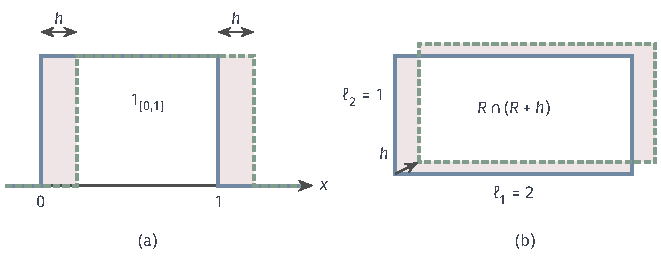
\includegraphics[width=112mm]{figures/04-spaces-measures-and-geometry/02-measure/tikz/weakd-translation/figure.pdf}
  \caption{平移引起的积分误差。蓝色实线为原函数或原矩形，绿色虚线为平移后的结果，红色区域是两者不相同的部分。(a)~$\mathbf 1_{[0,1]}$平移$h=0.2$，两侧条带上逐点误差都是$1$，积分误差为$2h=0.4$。(b)~二维矩形$R$平移$h=(0.2,0.1)$，红色部分是对称差，面积$0.76$。}
  \label{fig:weakd-translation}
\end{BookInlineFigure}

有了矩形的情形，就可以处理一般的可积函数：用矩形的有限并逼近，逼近误差和平移误差分开估计。

\begin{theorem}[平移的积分连续性]
\label{thm:weakd-translation-continuity}
设$F$在$\mathbb R^d$上可积。则
\begin{equation}
\omega_F(h):=\int_{\mathbb R^d}\lvert F(x-h)-F(x)\rvert\,\mathrm dx\to0\qquad(h\to0).
\label{eq:weakd-translation-modulus}
\end{equation}
\end{theorem}

\begin{proof}
任给$\eta>0$。第一步，用阶梯函数逼近$F$。对$F$的实部、虚部的正部与负部分别取递增的非负简单函数逼近，由单调收敛定理，可以得到简单函数$s$，满足$\int\lvert F-s\rvert<\eta$。把$s$写成不同非零值的标准形式
\[
s=\sum_{i=1}^mc_i\mathbf 1_{A_i},
\]
其中$A_i$互不相交。$s$可积，所以每个$\lambda_d(A_i)<\infty$。

由式~\eqref{eq:weakd-box-approx}，对每个$i$取矩形的有限并$E_i$，使$\lambda_d(A_i\triangle E_i)<\eta/(m\lvert c_i\rvert)$，并令$u=\sum_ic_i\mathbf 1_{E_i}$。两个指示函数之差的绝对值正是对称差的指示函数，所以$\int\lvert s-u\rvert<\eta$，从而
\[
\int\lvert F-u\rvert\,\mathrm dx<2\eta .
\]

第二步，比较三项。由三角不等式，
\[
\begin{aligned}
\lvert F(x-h)-F(x)\rvert\leq{}&\lvert F(x-h)-u(x-h)\rvert+\lvert u(x-h)-u(x)\rvert\\
&+\lvert u(x)-F(x)\rvert .
\end{aligned}
\]
对$x$积分。第一项由平移规则~\eqref{eq:weakd-translation-scaling}等于$\int\lvert F-u\rvert$，于是
\[
\omega_F(h)<4\eta+\omega_u(h).
\]

第三步，估计$\omega_u(h)$。设$E_i=R_{i,1}\cup\cdots\cup R_{i,N_i}$。若$\mathbf 1_{E_i}(x-h)\neq\mathbf 1_{E_i}(x)$，则$x-h$与$x$中恰有一个属于$E_i$，属于的那个落在某个$R_{i,k}$中而另一个不在其中，所以
\[
\lvert\mathbf 1_{E_i}(x-h)-\mathbf 1_{E_i}(x)\rvert\leq\sum_{k=1}^{N_i}\lvert\mathbf 1_{R_{i,k}}(x-h)-\mathbf 1_{R_{i,k}}(x)\rvert .
\]

积分并乘以$\lvert c_i\rvert$求和，得到
\[
\omega_u(h)\leq\sum_i\lvert c_i\rvert\sum_k\omega_{\mathbf 1_{R_{i,k}}}(h).
\]
这是有限和，由式~\eqref{eq:weakd-box-translation}，右端随$h\to0$趋于零。因此$h$足够小时$\omega_F(h)<5\eta$，而$\eta$任意。
\end{proof}

定理只控制积分误差，不控制逐点误差。图~\ref{fig:weakd-translation}(a)中对每个$h\neq0$都有点使误差等于$1$，而积分误差是$2\lvert h\rvert$，这种差别在阶跃函数上不会消失。下一小节需要的恰好只是积分误差。

\subsection{磨光的局部逼近}
\label{sec:weakd-local-approximation}

现在回到磨光函数。我们只在离边界有正距离的紧集上比较$f_\varepsilon$与$f$，因为靠近边界时磨光半径必须随之缩小。思路是把$f$截成一个可积函数，使磨光在紧集上只读取这个截断函数，然后把误差写成平移误差的平均。

\begin{theorem}[磨光的局部积分逼近]
\label{thm:weakd-local-approximation}
设$f\in L^1_{\mathrm{loc}}(\Omega)$，$K\subset\Omega$是非空紧集，$\delta=\operatorname{dist}(K,\Omega^{c})>0$。则当$0<\varepsilon<\delta$时$K\subset\Omega_\varepsilon$，并且
\begin{equation}
\int_K\lvert f_\varepsilon(x)-f(x)\rvert\,\mathrm dx\to0\qquad(\varepsilon\to0).
\label{eq:weakd-local-approximation}
\end{equation}
\end{theorem}

\begin{proof}
令$\delta_0=\min\{\delta,1\}$，这样$\Omega=\mathbb R^d$时$\delta=+\infty$的情形也包括在内。再令
\[
K'=\{x:\operatorname{dist}(x,K)\leq\delta_0/2\}.
\]
$K'$是有界闭集，并且离$\Omega^{c}$至少$\delta_0/2$，所以是$\Omega$内的紧集。令$F=f\mathbf 1_{K'}$，并在$\Omega$外取零，则$F$在$\mathbb R^d$上可积。这正是图~\ref{fig:weakd-interior}(b)的设置。

当$x\in K$、$\varepsilon<\delta_0/2$、$\lvert z\rvert\leq\varepsilon$时，$x-z\in K'$，所以$f(x-z)=F(x-z)$，并且$f(x)=F(x)$。利用$\int\rho_\varepsilon=1$把$f(x)$也写成平均，得到
\[
f_\varepsilon(x)-f(x)=\int_{\lvert z\rvert\leq\varepsilon}\rho_\varepsilon(z)\bigl(F(x-z)-F(x)\bigr)\,\mathrm dz ,\qquad x\in K .
\]

取绝对值、对$x\in K$积分，再对非负被积函数用Tonelli定理交换次序，得
\[
\begin{aligned}
\int_K\lvert f_\varepsilon-f\rvert\,\mathrm dx
&\leq\int_{\lvert z\rvert\leq\varepsilon}\rho_\varepsilon(z)\Bigl(\int_{\mathbb R^d}\lvert F(x-z)-F(x)\rvert\,\mathrm dx\Bigr)\mathrm dz\\
&\leq\sup_{\lvert z\rvert\leq\varepsilon}\omega_F(z).
\end{aligned}
\]
最后一步用了$\rho_\varepsilon\geq0$与$\int\rho_\varepsilon=1$：非负权重的平均不超过被平均量的上确界。由定理~\ref{thm:weakd-translation-continuity}，右端随$\varepsilon\to0$趋于零。
\end{proof}

证明的关键是核非负且积分为$1$：误差$f_\varepsilon-f$本身就是平移误差的加权平均，权重的总量为$1$，所以平均误差被最坏的小平移误差控制。若核取负值，权重绝对值的总积分可能大于$1$，同样的估计要多出一个因子；若核的积分不为$1$，常数函数的磨光就不再等于自身。

\begin{example}[阶跃函数的磨光误差]
\label{ex:weakd-step-mollification}
在$\Omega=(-1,1)$上取$H=\mathbf 1_{(0,1)}$，$K=[-1/2,1/2]$，并设$\varepsilon<1/2$。由式~\eqref{eq:weakd-mollification}，对$x\in K$有
\[
H_\varepsilon(x)=\int_{z<x}\rho_\varepsilon(z)\,\mathrm dz .
\]
所以在$x\leq-\varepsilon$处$H_\varepsilon=0$，在$x\geq\varepsilon$处$H_\varepsilon=1$，只在$(-\varepsilon,\varepsilon)$内取中间值。积分误差只来自这一段：
\[
\int_K\lvert H_\varepsilon-H\rvert\,\mathrm dx=\int_{-\varepsilon}^0H_\varepsilon\,\mathrm dx+\int_0^\varepsilon(1-H_\varepsilon)\,\mathrm dx .
\]

核是偶函数，所以$H_\varepsilon(-x)=1-H_\varepsilon(x)$，上式两项相等。又$x>0$时，$1-H_\varepsilon(x)$就是$\rho_\varepsilon$在$[x,\varepsilon]$上的积分，用Tonelli定理交换次序，得到
\[
\int_0^\varepsilon\!\!\int_x^\varepsilon\rho_\varepsilon(z)\,\mathrm dz\,\mathrm dx
=\int_0^\varepsilon z\,\rho_\varepsilon(z)\,\mathrm dz
=\frac{\varepsilon m_1}{2}.
\]
两项相加，积分误差恰好是
\[
\int_K\lvert H_\varepsilon-H\rvert\,\mathrm dx=\varepsilon m_1 .
\]
$\varepsilon=0.5,0.25,0.1$时分别约为$0.167,0.084,0.033$。

另一方面，核的对称性给出$H_\varepsilon(0)=\tfrac12$。当$x\to0^+$时$H_\varepsilon(x)\to\tfrac12$而$H(x)=1$，所以误差的上确界不小于$\tfrac12$；又在$K$上处处有$\lvert H_\varepsilon-H\rvert\leq\tfrac12$，因此上确界恰为$\tfrac12$，与$\varepsilon$无关。
\end{example}

图~\ref{fig:weakd-step-error}对比了这两种误差。曲线越来越陡，积分误差线性地趋于零；但最大误差始终停在$\tfrac12$，因为光滑函数要连续地穿过跳跃。

\begin{BookInlineFigure}
  \centering
  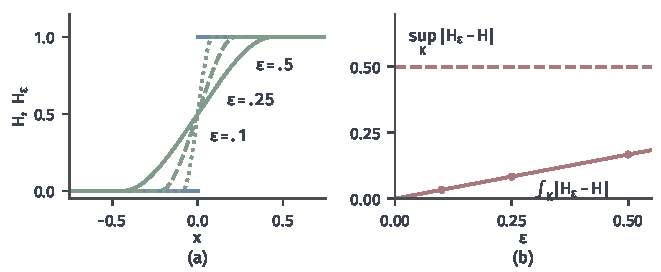
\includegraphics[width=112mm]{figures/04-spaces-measures-and-geometry/02-measure/matplotlib/weakd-step-error/figure.pdf}
  \caption{阶跃函数的磨光误差。(a)~蓝色为阶跃函数$H$，绿色为$H_\varepsilon$，$\varepsilon=0.5,0.25,0.1$依次由实线、虚线、点线表示，三条曲线都通过$(0,\tfrac12)$。(b)~$K=[-\tfrac12,\tfrac12]$上的两种误差：积分误差$\varepsilon m_1$（实线，圆点对应三个$\varepsilon$）随$\varepsilon$线性趋零，最大误差（虚线）保持为$\tfrac12$。}
  \label{fig:weakd-step-error}
\end{BookInlineFigure}

\subsection{测试函数判别}
\label{sec:weakd-test-criterion}

有限维空间里，判断一个向量是否为零，可以逐个看它在基向量上的分量：若$\langle v,e_k\rangle=0$对每个$k$成立，则$v=0$。函数的情形有类似的问题：若$h$与每个测试函数相乘后的积分都为零，$h$是否为零？

类比要作一处调整。函数“在一点的分量”$h(x)$无法用积分读出，因为单点没有测度；测试函数是一支有宽度的探针，读到的是$h$在一小块区域上的加权平均。图~\ref{fig:weakd-test-probe}说明单支探针可能什么都读不到：宽探针同时盖住正负两部分，读数为零；把探针收窄到正的部分，读数就变成正数。

\begin{BookInlineFigure}
  \centering
  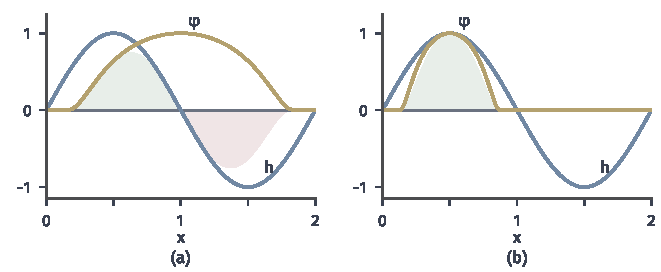
\includegraphics[width=112mm]{figures/04-spaces-measures-and-geometry/02-measure/matplotlib/weakd-test-probe/figure.pdf}
  \caption{测试函数作为探针。蓝色为$h(x)=\sin\pi x$，黄色为测试函数$\varphi$，填充部分是乘积$h\varphi$，绿色为正、红色为负。(a)~$\varphi$以$x=1$为中心、半径$0.9$，正负部分相消，$\int h\varphi=0$。(b)~$\varphi$以$x=0.5$为中心、半径$0.4$，$\int h\varphi\approx0.425$。}
  \label{fig:weakd-test-probe}
\end{BookInlineFigure}

积分看不见零测集上的差别，所以至多能期望几乎处处为零。磨光给出了肯定的回答，因为磨光值本身就是一个测试积分。

\begin{theorem}[测试函数判别]
\label{thm:weakd-test-criterion}
设$h\in L^1_{\mathrm{loc}}(\Omega)$，且对所有$\varphi\in C_c^\infty(\Omega)$都有$\int_\Omega h\varphi\,\mathrm dx=0$。则$h=0$在$\Omega$上几乎处处成立。
\end{theorem}

\begin{proof}
固定$\varepsilon>0$与$x\in\Omega_\varepsilon$。函数$\varphi_x(y)=\rho_\varepsilon(x-y)$光滑，支撑是闭球$\overline B(x,\varepsilon)$，它紧且含于$\Omega$，所以$\varphi_x\in C_c^\infty(\Omega)$。由假设，
\[
h_\varepsilon(x)=\int_\Omega h\,\varphi_x\,\mathrm dy=0 .
\]
也就是说，$h_\varepsilon$在$\Omega_\varepsilon$上恒为零。

取紧集$K\subset\Omega$。当$\varepsilon<\operatorname{dist}(K,\Omega^{c})$时，由定理~\ref{thm:weakd-local-approximation}，
\[
\int_K\lvert h\rvert\,\mathrm dx=\int_K\lvert h-h_\varepsilon\rvert\,\mathrm dx\to0 .
\]
左端与$\varepsilon$无关，所以$\int_K\lvert h\rvert=0$，即$h=0$在$K$上几乎处处成立。

最后用可数个紧集填满$\Omega$。令
\[
K_m=\{x\in\Omega:\lvert x\rvert\leq m,\ \operatorname{dist}(x,\Omega^{c})\geq1/m\},\qquad m=1,2,\ldots .
\]
它们是$\Omega$内的紧集，并且并集为$\Omega$：每个$x\in\Omega$到补集的距离为正，$m$足够大时$x\in K_m$。可数个零测集之并仍是零测集，所以$h=0$在$\Omega$上几乎处处成立。
\end{proof}

最后一步不能省。每个紧集上的结论只排除该紧集上的非零部分；开集一般不是紧集，需要用可数个内部紧集把它填满，并依靠可数可加性把各处的零测例外合在一起。复值的$h$不需要分开实部与虚部，因为定理~\ref{thm:weakd-local-approximation}对复值函数同样成立。

把判别法用于两个函数之差，就得到识别结论：若$f,g\in L^1_{\mathrm{loc}}(\Omega)$对所有测试函数满足$\int f\varphi=\int g\varphi$，则$f=g$几乎处处。因此，一个局部可积函数的几乎处处等价类，完全由它与全部测试函数的积分值决定，正如有限维向量由它在基上的分量决定。这一结论将保证下一节的弱导数不会有两个本质不同的候选。
